\item Determine a altura $h$ da rampa $D$ que o carrinho da montanha-russa de \SI{200}{\kilogram} atingirá se for lançado em $B$ com uma velocidade apenas suficiente para dar a volta no topo de \textit{loop} em $C$ sem deixar os trilhos. O raio de curvatura em $C$ é $\rho_{C}=\SI{25}{\meter}$.

\import{answers/}{answer-5}

\vspace{-1.5cm}
\begin{flushright}
    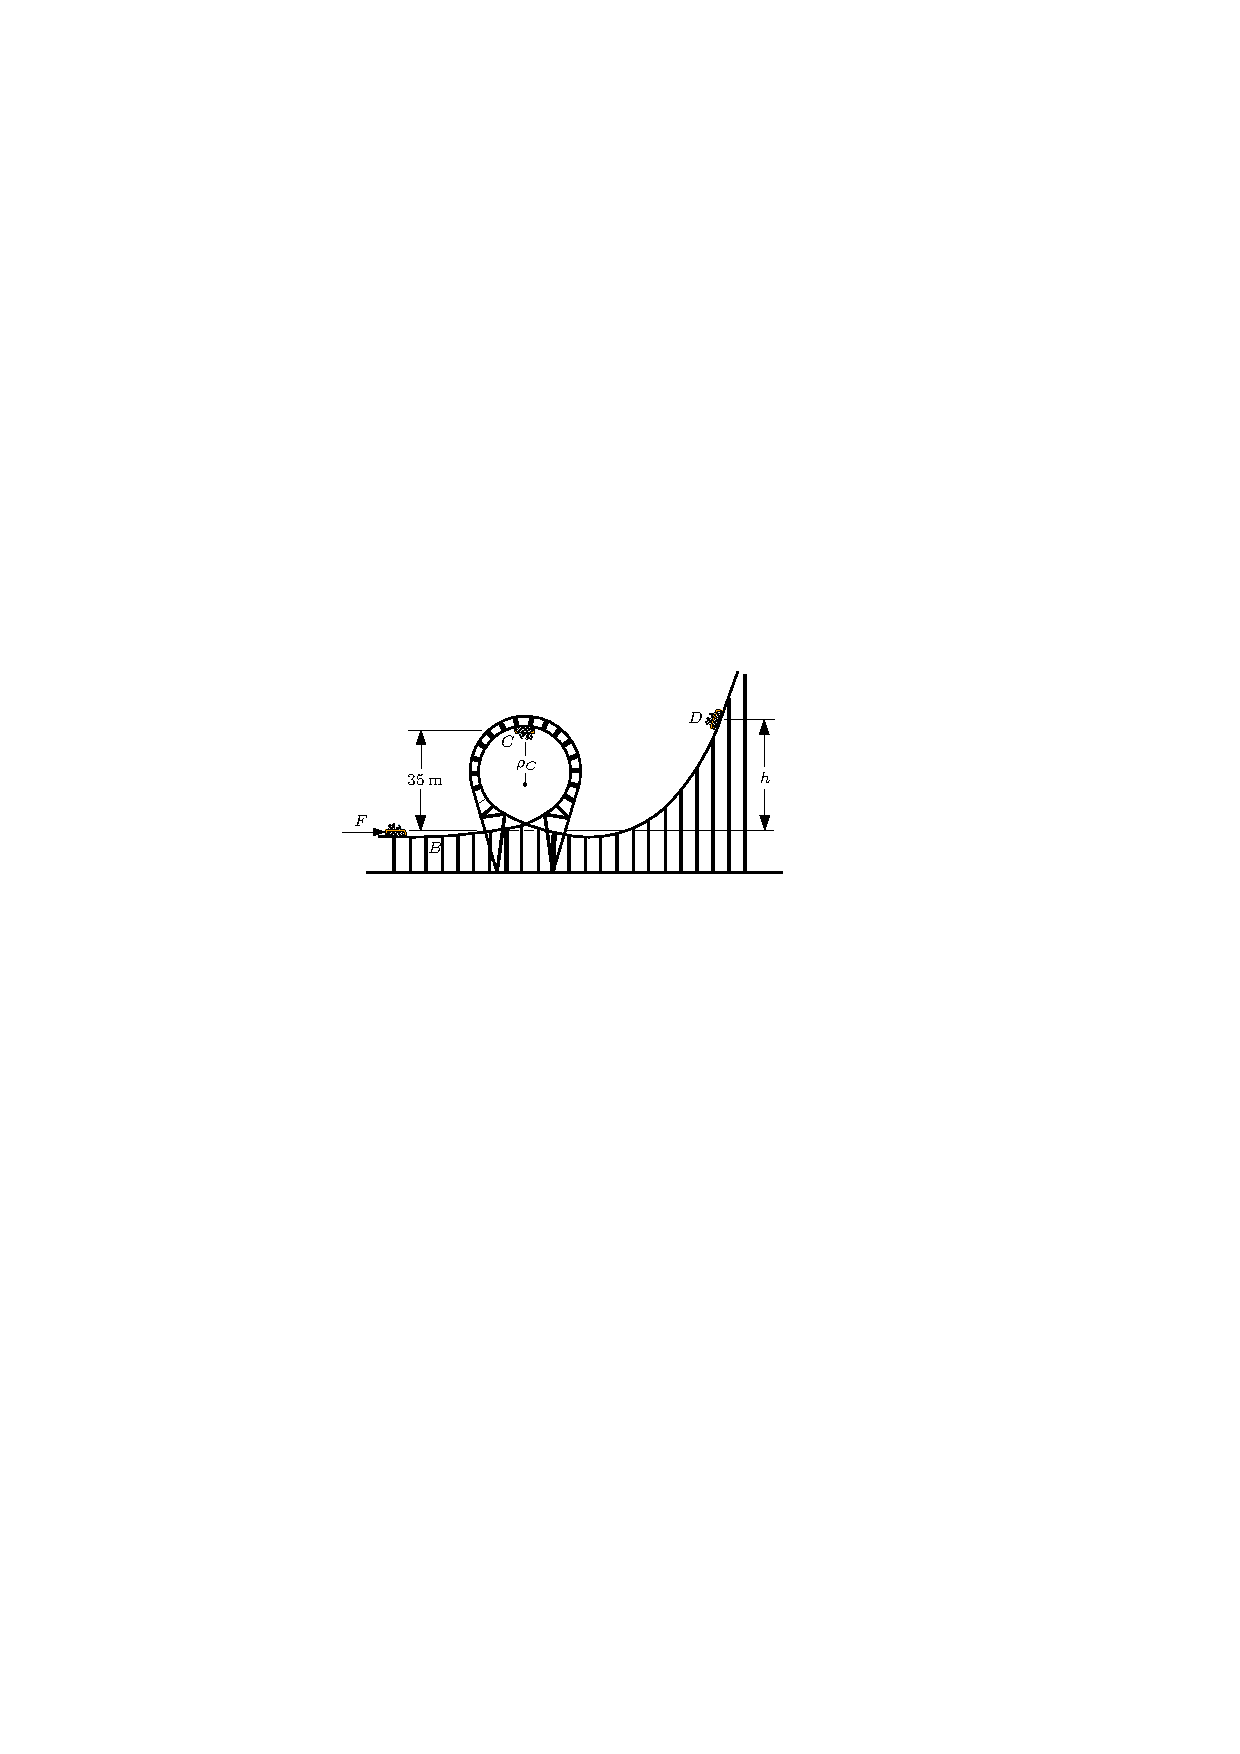
\includegraphics[scale=1.8]{images/draw_5.pdf}
\end{flushright}
